\documentclass[11pt,a4paper]{article}
\usepackage[margin=23mm]{geometry}
\usepackage[T1]{fontenc}
\usepackage{lmodern}
\usepackage{amsmath,amssymb,amsthm,booktabs,longtable,array}
\usepackage{pgfplots}
\pgfplotsset{compat=1.18}
\usepackage{hyperref,enumitem,caption,fancyhdr}
\usepackage[section]{placeins}
\definecolor{navy}{RGB}{40,100,130}
\definecolor{rust}{RGB}{169,87,40}
\hypersetup{colorlinks=true,linkcolor=navy,urlcolor=navy,citecolor=navy,pdftitle={Bargaining Experience and Reciprocity: An eBay Pilot}}
\setlength{\parskip}{5pt}
\setlength{\parindent}{0pt}
\setlength{\tabcolsep}{4pt}
\renewcommand{\arraystretch}{1.18}
\setlist{itemsep=2pt,topsep=4pt}
\captionsetup{font=small,labelfont=bf}
\pagestyle{fancy}\fancyhf{}\fancyhead[L]{\small Bargaining experience and reciprocity}\fancyhead[R]{\small Empirical pilot}\fancyfoot[C]{\thepage}
\setlength{\headheight}{14pt}
\newtheorem{proposition}{Proposition}
\title{\textbf{Bargaining Experience and Reciprocity}\\[5pt]\large A fixed-stage eBay pilot with seller-level validation\\and an exploratory measurement comparison}
\author{nakshatra0904}
\date{11 October 2026\quad |\quad Version 1.1}
\begin{document}
\maketitle
\begin{abstract}
I investigate whether bargaining experience changes the strength of
reciprocal concession-making, rather than only the average concession level.
Using 30,419 actual four-offer eBay Best Offer threads from 4,520 sellers in a
nonrandom public-data prefix, I estimate a fixed-stage experience-by-concession
interaction. The primary novice/experienced contrast uses 27,016 threads and
3,004 seller clusters. Its interaction is 0.0127 (clustered SE 0.0587,
95\% CI $[-0.1023,0.1277]$, p=0.829); a seller-level split and planned checks
do not establish weaker reciprocity among experienced sellers. A benchmark
response slope is positive for remaining-gap fractions, 0.090, but negative
for price movements on a common scale, $-0.097$. This exploratory sign
disagreement recurs across the seller split. An algebraic derivation shows
why these different parameters can have opposite signs. The proposed
contribution is an experience-response extension and a transparent measurement
diagnostic, not a causal effect, a refutation of the literature, or verified
publication-level novelty.
\end{abstract}
\textbf{Reading guide.} The main text explains the design and interpretation.
Tables report all planned and exploratory focal estimates. Four figures show
validation, robustness, selection and measurement sensitivity. Appendices
include every planned-model coefficient and the graph data. All numerical
outputs are consolidated in \texttt{results/results.json}; the LaTeX source
contains its figures and references inline.
\clearpage
\tableofcontents
\clearpage
\section{Research question and contribution}
Online bargaining records make it possible to observe both prices and the
offer sequence. I study the buyer's first counteroffer and the
seller's following counteroffer at the same stage across threads. The original
interest was bargaining on ride platforms; I use eBay because
the public archive supplies actual offer histories. It contains no inDrive data.

The question is: \emph{does experience change how strongly a seller responds
to an opponent's concession?} Conceding less on average and being less
responsive to a buyer's new concession are different empirical claims.

Backus, Blake, Larsen and Tadelis (2020) study reciprocity and experience-related
concession levels in eBay data. Their appendix already considers alternative
percentage-concession measures. Fong and Waisman (2025) use an instrumental-variable
design to study delay. These findings motivate my empirical question;
I do not reproduce those papers' exact samples or identification in this pilot.

\subsection{What is an extension, and what is already established?}
\begin{enumerate}
\item \textbf{Existing foundation:} reciprocal concession patterns, bargaining
experience and their relation to concession levels have been studied before.
Comparing bargaining rounds alone or checking an alternative scale alone
would not be a new contribution.
\item \textbf{Proposed extension:} interact the opponent's concession with
seller experience at one fixed stage. I distinguish slope heterogeneity from
average toughness and examine the same pre-set contrast on disjoint seller halves.
\item \textbf{Additional exploratory diagnostic:} document and explain a
measurement discrepancy within the completed pilot. The common-price check
was planned; its seller-split follow-up followed the observed disagreement.
\end{enumerate}
My targeted literature search did not establish that the exact interaction
design had already been published. This is a candidate student-project
extension; I do not claim certified global novelty. I retain the null primary
result and report all planned tests.

\section{A simple response model and testable hypothesis}
Let $x\in[0,1]$ denote the buyer's concession and $q\in[0,1]$ the seller's
following concession, each as a fraction of its relevant price gap. I use
the following illustrative reduced-form behavioral loss
\begin{equation}
L(q;e,x)=\frac{c}{2}[q-m(e)]^2+\frac{\rho(e)}{2}(q-x)^2,
\qquad c>0,\quad\rho(e)>0.\label{eq:loss}
\end{equation}
Here $m(e)$ is a preferred concession without the matching motive, and
$\rho(e)$ is the weight on matching the opponent's concession. This is an
illustrative response model, not a full alternating-offers equilibrium.
\begin{proposition}
For $m(e),x\in[0,1]$, the unique minimizer is
\[
q^*(e,x)=\frac{c\,m(e)+\rho(e)x}{c+\rho(e)}.
\]
Its response slope is positive. Holding $c$ fixed, an experience-related
decline in $\rho$ reduces that slope, whereas a decline in $m$ can reduce
concession levels without changing the slope.
\end{proposition}
\begin{proof}
The first-order condition is $c(q-m)+\rho(q-x)=0$ and the second derivative
is $c+\rho>0$. The solution is a convex combination of $m$ and $x$, so it is
feasible. Differentiation gives
\[
\frac{\partial q^*}{\partial x}=\frac{\rho(e)}{c+\rho(e)}>0,\qquad
\frac{\partial^2q^*}{\partial e\,\partial x}
=\frac{c\rho'(e)}{[c+\rho(e)]^2}.
\]
The intercept component can change through $m$ while the slope stays fixed.
\end{proof}
My directional hypothesis recorded before inspecting sample outcomes was
that experienced sellers have a weaker response slope. Observational data
cannot separately identify $c$, $m$ and $\rho$, or attribute a slope to a
reciprocity motive rather than strategic response or selection.

\section{Data and sample construction}
\subsection{Public source, period and bounded download}
I use the NBER anonymized eBay bargaining archive. I retained exactly the
first 67,108,864 compressed bytes (64 MiB) with a byte-range download.
It produced 2,234,913 offer rows, 1,324,190 thread IDs and 21,315 sellers.
Observed offer timestamps span June 2012--December 2013. The sample is a
contiguous, seller-grouped prefix, not a random or representative draw.
I discarded the final seller block because the range may end mid-history.
The download manifest records the range, source and checksum.

\subsection{History filters and the fixed stage}
I remove identical analysis-field records, inconsistent party identifiers,
conflicting timestamps, non-alternating sequences, nonpositive prices, missing
initial experience and automatic acceptance/rejection histories. Pre-terminal
offers must have the source countered status. Histories are chronologically
ordered, contain at most six offers, and require each observable interior
concession to lie between the preceding offers. These restrictions select
a subset; they are not the original paper's exact cleaning procedure.
\begin{table}[htbp]
\centering\small
\caption{Sequential sample construction}\label{tab:flow}
\begin{tabular}{p{7.1cm}rrr}
\toprule
Filter / sample & Offer rows & Threads & Sellers \\
\midrule
Raw prefix & 2,234,913 & 1,324,190 & 21,315 \\
Drop potentially truncated last seller & 2,227,948 & 1,320,212 & 21,314 \\
Deduplicate identical analysis-field records & 2,227,877 & 1,320,212 & 21,314 \\
Strict alternating human offer histories & 1,363,663 & 928,563 & 18,614 \\
Observed initial experience for both parties & 1,315,115 & 900,435 & 18,554 \\
Every observed interior concession bounded in [0,1] & 1,304,538 & 897,890 & 18,542 \\
Incoming qualifying buyer offers & -- & 70,167 & -- \\
Four-offer analysis sample & -- & 30,419 & 4,520 \\
Primary experience contrast & -- & 27,016 & 3,004 \\
\bottomrule
\end{tabular}
\par\vspace{4pt}\begin{minipage}{\linewidth}\footnotesize The first six rows are sequential history filters. The last three rows select fixed-stage analytical samples. The raw prefix is nonrandom; the last seller block is removed because it may be truncated.\end{minipage}
\end{table}

The fixed stage consists of four prices: $B_1$ (initial buyer offer),
$S_2$ (first seller counteroffer), $B_3$ (first buyer counteroffer), and
$S_4$ (second seller counteroffer). Define
\begin{equation}
x=\frac{B_3-B_1}{S_2-B_1},\qquad
q=\frac{S_2-S_4}{S_2-B_3},\qquad
d=\frac{S_2-B_1}{S_2}.\label{eq:measures}
\end{equation}
Qualifying histories have positive denominators and $x,q\in[0,1]$.
For illustration only, $B_1=60$, $S_2=100$, $B_3=80$, $S_4=90$ imply
$x=q=0.5$. This numerical example is not an observation used in estimation.
\begin{table}[htbp]
\centering\small
\caption{Descriptive statistics by recorded seller experience}\label{tab:desc}
\begin{tabular}{lrrrrr}
\toprule
Experience & Threads & Sellers & Buyer mean & Seller mean & Median $S_2$ \\
\midrule
0-9 & 742 & 640 & 35.70 & 26.43 & 167.50 \\
10-99 & 3,403 & 1,873 & 34.89 & 25.51 & 120.00 \\
100+ & 26,274 & 2,385 & 35.63 & 23.18 & 60.00 \\
\bottomrule
\end{tabular}
\par\vspace{4pt}\begin{minipage}{\linewidth}\footnotesize Concession means are percentages of the relevant price gap; prices use the source price units. Some sellers cross experience thresholds over time, so seller counts need not sum to the unique total. The observed minimum experience count is 1.\end{minipage}
\end{table}

\subsection{Experience definition and seller split}
The codebook describes experience as previous threads, while the paper's
Table I discussion describes a count including the current thread. I use
the supplied count unchanged and label thresholds as recorded experience.
The observed minimum is 1; the pre-set novice bin is below 10 and the
experienced bin is at least 100. Counts 10--99 remain in descriptive and
common-slope analyses but are excluded from the primary contrast.
Some sellers cross thresholds over time; group seller counts therefore need
not sum to the unique total.

Before fitting, I split seller IDs by SHA-256: the integer represented by
the first eight hexadecimal digits determines the half by parity. No seller
appears in both halves. Buyers can appear in both halves, and the comparison
is a seller-level stability check, not a fully independent population experiment.

\section{Regression specifications and uncertainty}
\subsection{Primary interaction}
For the fixed-stage qualifying continuers, I estimate
\begin{equation}
q_i=\alpha+\beta x_i+\theta E_i+\delta(x_iE_i)
+X_i'\eta+\mu_{m(i)}+\varepsilon_i.\label{eq:primary}
\end{equation}
$E_i=1$ for a recorded seller count of at least 100; the reference count is
below 10. $X_i$ contains log(1 + buyer experience), log $S_2$ and $d$ before
the buyer's concession. Calendar-month effects use the initial offer month.
I implement ordinary least squares as weighted least squares with unit
weights. For the equal-seller check, I use inverse within-sample seller thread
counts. For the seller fixed-effects check, I demean within seller and absorb
seller intercepts.

The novice slope is $\beta$, the experienced slope is $\beta+\delta$, and
$\delta$ is the focal difference. Seller-clustered covariance allows correlated
errors across a seller's threads. Intervals and two-sided p-values use the
cluster-count t reference. The fixed-effects variance adjustment also counts
absorbed seller intercepts. It does not solve omitted slope heterogeneity.

\subsection{Benchmark and measurement follow-up}
I estimate the benchmark using all experience categories, continuous log(1 + seller
experience), the buyer experience/price/gap controls, and month effects.
In the measurement follow-up, I keep these controls and threads fixed but change
the exposure/outcome definitions. It includes gap fractions; both price
movements divided by $S_2$; and percentages of each party's own preceding price.
I do not claim causal identification or apply a multiplicity adjustment.

\section{Primary results and validation}
\begin{table}[htbp]
\centering\small
\caption{Primary OLS interaction regressions}\label{tab:main}
\begin{tabular}{p{7.1cm}rrr}
\toprule
Variable & All & Discovery & Validation \\
\midrule
Buyer concession ($\beta$) & \shortstack{0.0716\\(0.0539)} & \shortstack{0.0337\\(0.0739)} & \shortstack{0.1020\\(0.0788)} \\
Experienced indicator ($\theta$) & \shortstack{-0.0359\\(0.0218)} & \shortstack{-0.0491\\(0.0308)} & \shortstack{-0.0251\\(0.0308)} \\
Buyer concession $\times$ experience ($\delta$) & \shortstack{0.0127\\(0.0587)} & \shortstack{0.0452\\(0.0821)} & \shortstack{-0.0113\\(0.0833)} \\
Log(1 + buyer experience) & \shortstack{0.0007\\(0.0016)} & \shortstack{-0.0005\\(0.0022)} & \shortstack{0.0019\\(0.0022)} \\
Log first seller counteroffer ($S_2$) & \shortstack{0.0028\\(0.0028)} & \shortstack{0.0001\\(0.0034)} & \shortstack{0.0057\\(0.0043)} \\
Gap before buyer concession & \shortstack{-0.0189\\(0.0264)} & \shortstack{0.0121\\(0.0392)} & \shortstack{-0.0504\\(0.0332)} \\
Constant & \shortstack{0.2185\\(0.0270)} & \shortstack{0.2314\\(0.0380)} & \shortstack{0.2093\\(0.0385)} \\
Month fixed effects & Yes & Yes & Yes \\
Threads & 27,016 & 13,550 & 13,466 \\
Seller clusters & 3,004 & 1,487 & 1,517 \\
Interaction p-value & 0.829 & 0.582 & 0.893 \\
\bottomrule
\end{tabular}
\par\vspace{4pt}\begin{minipage}{\linewidth}\footnotesize Dependent variable: seller remaining-gap concession $q$. Parentheses contain seller-clustered standard errors. Reference experience count: below 10; experienced: at least 100. Counts 10--99 are excluded. Month reference: June 2012. No significance stars are used; focal p-values and intervals are reported explicitly.\end{minipage}
\end{table}

I estimate an interaction of $0.0127$ with clustered SE $0.0587$, 95\% CI
$[-0.1023,0.1277]$ and p=0.829. A 10 percentage point larger buyer concession
therefore has an experienced-minus-novice response difference of $+0.13$
seller percentage points, with CI $[-1.02,1.28]$. The interval does not support
the proposed directional prediction, and it does not establish equivalence.

Discovery and validation estimates are $+0.0452$ and $-0.0113$, respectively;
both intervals include zero. The experience result is not stable evidence
of a stronger or weaker response.
\begin{figure}[htbp]\centering
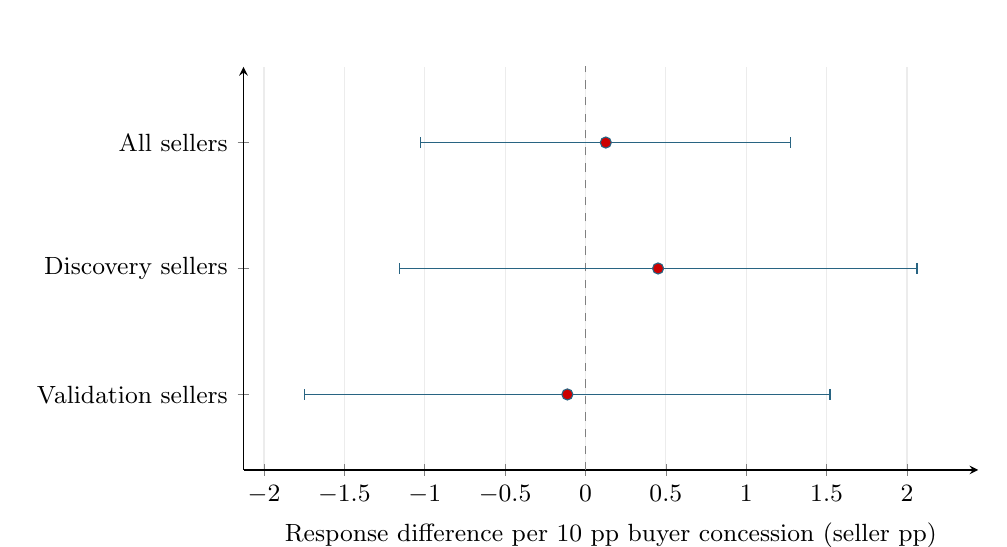
\begin{tikzpicture}\begin{axis}[width=.90\linewidth,height=6.7cm,xmin=-2.127245,xmax=2.443400,ymin=.4,ymax=3.6,ytick={3,2,1},yticklabels={{All sellers},{Discovery sellers},{Validation sellers}},axis lines=left,xmajorgrids=true,grid style={gray!15},tick label style={font=\small},xlabel style={font=\small},ylabel style={font=\small},scaled x ticks=false,xticklabel style={/pgf/number format/fixed},xlabel={Response difference per 10 pp buyer concession (seller pp)},]\addplot[gray,dashed] coordinates {(0,0)(0,4)};\addplot+[only marks,mark=*,color=navy,error bars/.cd,x dir=both,x explicit] table[x=x,y=y,x error=err,row sep=\\]{x y err \\
0.12654405 3 1.15001157 \\
0.45176425 2 1.61074865 \\
-0.11253770 1 1.63381988 \\};\end{axis}\end{tikzpicture}
\caption{Primary experience interaction and seller-level validation.
Points are adjusted slope differences expressed as the seller response in
percentage points per 10 pp buyer concession. Whiskers are 95\% seller-clustered
intervals. Source: NBER eBay, June 2012--December 2013, nonrandom prefix.}
\label{fig:primary}\end{figure}

In the all-experience benchmark, I estimate a positive gap-fraction response
slope of $0.090$ (SE $0.0176$, CI $[0.055,0.124]$). A 10 pp larger buyer
concession is associated with a 0.90 pp larger seller concession. This
resembles the published pattern but is neither an exact coefficient replication
nor evidence that a norm caused it. Raw seller concession means are 26.43\%
for novices and 23.18\% for experienced sellers. That level difference is
descriptive; it does not establish an experience difference in response slopes.

\section{Planned robustness and continuation selection}
\begin{table}[htbp]
\centering\small
\caption{All eleven planned interaction specifications}\label{tab:checks}
\begin{tabular}{lp{4.0cm}rrrrr}
\toprule
ID & Specification & $N$ & $\delta$ & SE & 95\% CI & p \\
\midrule
M1 & All sellers & 27,016 & 0.0127 & 0.0587 & [-0.102, 0.128] & 0.829 \\
M2 & Discovery & 13,550 & 0.0452 & 0.0821 & [-0.116, 0.206] & 0.582 \\
M3 & Validation & 13,466 & -0.0113 & 0.0833 & [-0.175, 0.152] & 0.893 \\
M4 & Seller fixed effects & 27,016 & -0.0413 & 0.1116 & [-0.260, 0.178] & 0.711 \\
M5 & Experience 50+ & 28,462 & 0.0123 & 0.0583 & [-0.102, 0.127] & 0.833 \\
M6 & Experience 250+ & 24,395 & 0.0071 & 0.0595 & [-0.110, 0.124] & 0.905 \\
M7 & No messages & 12,203 & 0.0792 & 0.1122 & [-0.141, 0.299] & 0.480 \\
M8 & Price $1$--$1{,}000$ & 25,672 & 0.0318 & 0.0627 & [-0.091, 0.155] & 0.612 \\
M9 & Exclude midpoint / zero & 15,918 & -0.0292 & 0.0672 & [-0.161, 0.103] & 0.664 \\
M10 & Equal seller weights & 27,016 & 0.0110 & 0.0606 & [-0.108, 0.130] & 0.856 \\
M11 & Common-price scale & 27,016 & 0.0350 & 0.0286 & [-0.021, 0.091] & 0.221 \\
\bottomrule
\end{tabular}
\par\vspace{4pt}\begin{minipage}{\linewidth}\footnotesize M1--M10 use gap fractions. M11 scales both price movements by $S_2$ and estimates a different parameter. Confidence intervals are seller-clustered. None of these eleven planned interaction intervals excludes zero. The seller fixed-effects CR1 adjustment counts the absorbed seller intercepts conservatively.\end{minipage}
\end{table}

\begin{table}[htbp]
\centering\small
\caption{Group-specific slopes for every planned model}\label{tab:group}
\begin{tabular}{lrrrrrr}
\toprule
ID & Novice slope & SE & Experienced slope & SE & Novice $N$ & Exp. $N$ \\
\midrule
M1 & 0.0716 & 0.0539 & 0.0843 & 0.0214 & 742 & 26,274 \\
M2 & 0.0337 & 0.0739 & 0.0789 & 0.0337 & 351 & 13,199 \\
M3 & 0.1020 & 0.0788 & 0.0908 & 0.0250 & 391 & 13,075 \\
M4 & 0.1942 & 0.1097 & 0.1529 & 0.0182 & 742 & 26,274 \\
M5 & 0.0716 & 0.0539 & 0.0839 & 0.0205 & 742 & 27,720 \\
M6 & 0.0718 & 0.0540 & 0.0789 & 0.0232 & 742 & 23,653 \\
M7 & 0.0777 & 0.1078 & 0.1569 & 0.0279 & 219 & 11,984 \\
M8 & 0.0438 & 0.0579 & 0.0756 & 0.0224 & 649 & 25,023 \\
M9 & 0.2555 & 0.0655 & 0.2263 & 0.0157 & 404 & 15,514 \\
M10 & 0.0771 & 0.0564 & 0.0880 & 0.0232 & 742 & 26,274 \\
M11 & -0.1328 & 0.0287 & -0.0978 & 0.0129 & 742 & 26,274 \\
\bottomrule
\end{tabular}
\par\vspace{4pt}\begin{minipage}{\linewidth}\footnotesize Model IDs are defined in Table~\ref{tab:checks}. Experienced slope equals $\beta+\delta$, with its standard error calculated using the covariance between these terms. M11 has common-price rather than gap-fraction units.\end{minipage}
\end{table}

The planned experience checks include seller fixed effects, 50+/250+
thresholds, no message threads, prices $1$--$1{,}000$, exclusion of exact
midpoints and zero concessions, equal seller weights and common-price scaling.
All eleven planned interaction intervals include zero. Dropping messages
leaves only 219 novice threads; precision depends on the small novice group,
not only on the large total sample.
\begin{figure}[htbp]\centering
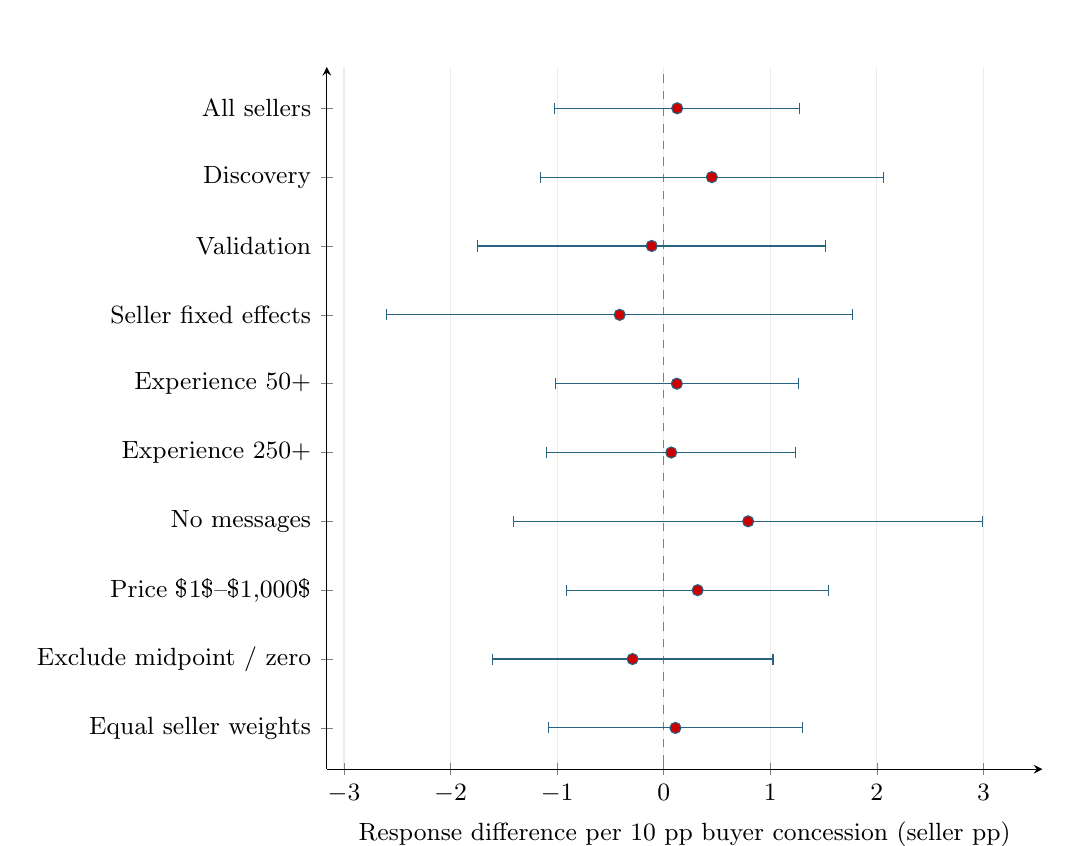
\begin{tikzpicture}\begin{axis}[width=.88\linewidth,height=10.5cm,xmin=-3.161549,xmax=3.553570,ymin=.4,ymax=10.6,ytick={10,9,8,7,6,5,4,3,2,1},yticklabels={{All sellers},{Discovery},{Validation},{Seller fixed effects},{Experience 50+},{Experience 250+},{No messages},{Price \$1\$--\$1{,}000\$},{Exclude midpoint / zero},{Equal seller weights}},axis lines=left,xmajorgrids=true,grid style={gray!15},tick label style={font=\small},xlabel style={font=\small},ylabel style={font=\small},scaled x ticks=false,xticklabel style={/pgf/number format/fixed},xlabel={Response difference per 10 pp buyer concession (seller pp)},]\addplot[gray,dashed] coordinates {(0,0)(0,11)};\addplot+[only marks,mark=*,color=navy,error bars/.cd,x dir=both,x explicit] table[x=x,y=y,x error=err,row sep=\\]{x y err \\
0.12654405 10 1.15001157 \\
0.45176425 9 1.61074865 \\
-0.11253770 8 1.63381988 \\
-0.41314599 7 2.18880963 \\
0.12317145 6 1.14208364 \\
0.07063703 5 1.16656700 \\
0.79241713 4 2.20155939 \\
0.31833839 3 1.22893710 \\
-0.29206824 2 1.31764775 \\
0.10969791 1 1.18858016 \\};\end{axis}\end{tikzpicture}
\caption{Planned gap-fraction interaction checks. Units are seller percentage
points per 10 pp buyer concession; whiskers are 95\% seller-clustered intervals.
Common-price scaling is omitted from this figure because its units differ,
but it is reported in Tables~\ref{tab:checks} and \ref{tab:group}.
Source: NBER eBay, June 2012--December 2013.}\label{fig:robust}\end{figure}

The secondary sample contains 70,167 qualifying incoming buyer counteroffers.
Higher-concession offers are often accepted, so no next seller counteroffer
is observed. The raw binned curves show this continuation selection; they
do not correct it. The outcome is responsiveness conditional on a qualifying
continued negotiation, not an unconditional response to every buyer offer.
\begin{figure}[htbp]\centering
\begin{minipage}{.49\linewidth}\centering\textbf{Continuing negotiations}\par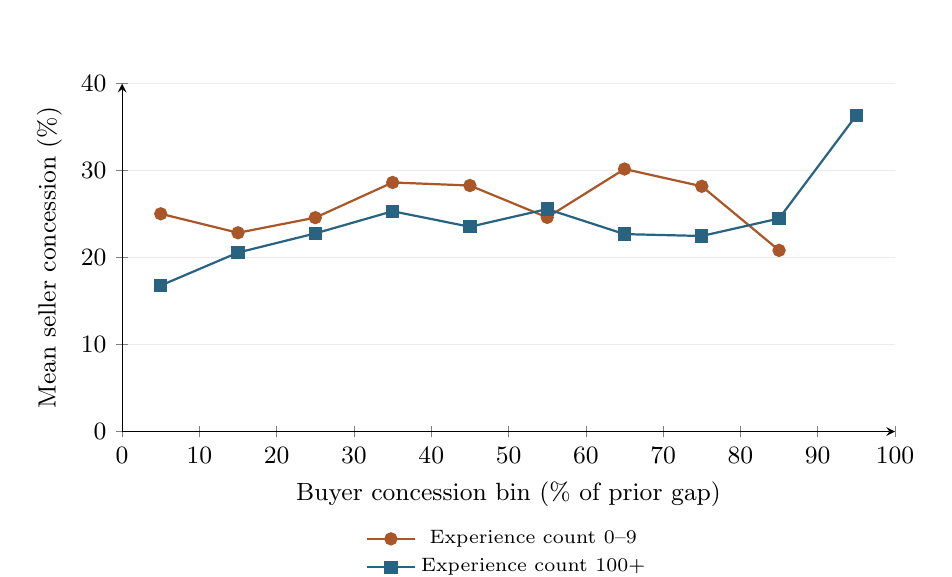
\begin{tikzpicture}\begin{axis}[width=.94\linewidth,height=6.0cm,xmin=0,xmax=100,ymin=0,ymax=40,xlabel={Buyer concession bin (\% of prior gap)},ylabel={Mean seller concession (\%)},axis lines=left,ymajorgrids=true,grid style={gray!15},tick label style={font=\small},label style={font=\small},legend style={font=\scriptsize,draw=none,at={(.5,-.25)},anchor=north,legend columns=1}]\addplot[color=rust,mark=*,thick] coordinates {(5.0,25.039304) (15.0,22.854858) (25.0,24.595620) (35.0,28.641515) (45.0,28.287616) (55.0,24.625591) (65.0,30.184748) (75.0,28.200923) (85.0,20.833333)};\addlegendentry{Experience count 0--9}\addplot[color=navy,mark=square*,thick] coordinates {(5.0,16.795213) (15.0,20.583053) (25.0,22.782068) (35.0,25.331595) (45.0,23.544715) (55.0,25.584695) (65.0,22.702424) (75.0,22.485853) (85.0,24.500457) (95.0,36.363636)};\addlegendentry{Experience count 100+}\end{axis}\end{tikzpicture}\end{minipage}\hfill\begin{minipage}{.49\linewidth}\centering\textbf{Incoming buyer offers}\par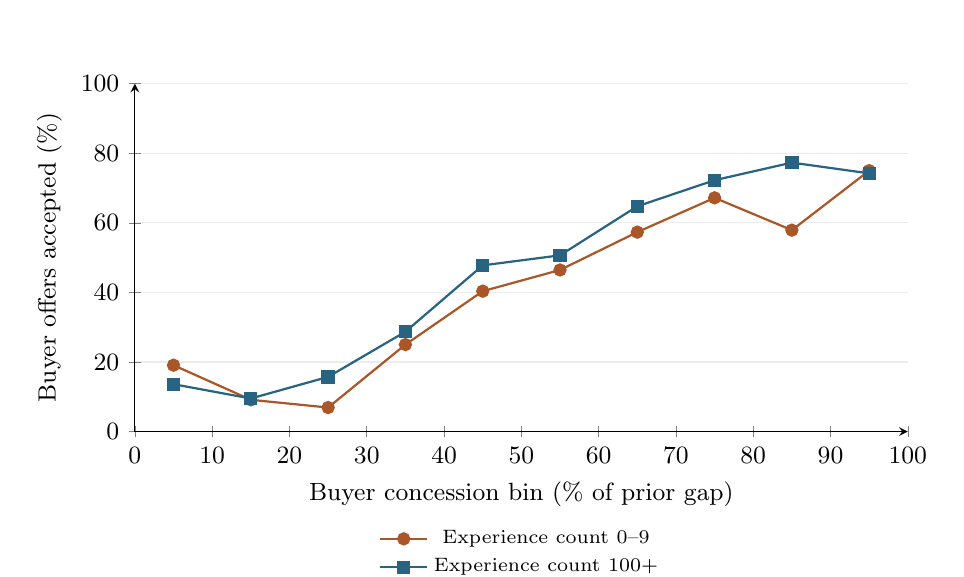
\begin{tikzpicture}\begin{axis}[width=.94\linewidth,height=6.0cm,xmin=0,xmax=100,ymin=0,ymax=100,xlabel={Buyer concession bin (\% of prior gap)},ylabel={Buyer offers accepted (\%)},axis lines=left,ymajorgrids=true,grid style={gray!15},tick label style={font=\small},label style={font=\small},legend style={font=\scriptsize,draw=none,at={(.5,-.25)},anchor=north,legend columns=1}]\addplot[color=rust,mark=*,thick] coordinates {(5.0,19.075145) (15.0,9.132420) (25.0,6.910569) (35.0,25.000000) (45.0,40.350877) (55.0,46.448087) (65.0,57.324841) (75.0,67.187500) (85.0,57.894737) (95.0,75.000000)};\addlegendentry{Experience count 0--9}\addplot[color=navy,mark=square*,thick] coordinates {(5.0,13.614341) (15.0,9.503136) (25.0,15.721097) (35.0,28.700118) (45.0,47.766990) (55.0,50.653880) (65.0,64.749418) (75.0,72.255575) (85.0,77.306273) (95.0,74.215553)};\addlegendentry{Experience count 100+}\end{axis}\end{tikzpicture}\end{minipage}
\caption{Raw concessions and response selection. Left: mean seller remaining-gap
concession among four-offer continuers. Right: fraction of incoming buyer
round-3 offers accepted. Points are 10 pp bins; groups use recorded experience.
High-concession novice bins are sparse (only four continuing threads at
80--90\% and none at 90--100\%). Source: NBER eBay, June 2012--December 2013.}
\label{fig:selection}\end{figure}

\section{Exploratory measurement discrepancy}
Using the same 30,419 threads and benchmark controls, I find a positive slope for gap
fractions, $+0.090$ with CI $[0.055,0.124]$, and a negative slope when both
price movements are divided by $S_2$, $-0.097$ with CI $[-0.120,-0.075]$.
The validation half reproduces the sign disagreement: $+0.096$ versus $-0.088$.
These definitions estimate different parameters.
\small
\begin{longtable}{p{4.3cm}lrrrrr}
\caption{Exploratory common-slope measurement comparisons}\label{tab:measure}\\
\toprule
Measure & Sample & $N$ & Slope & SE & 95\% CI & p \\
\midrule\endfirsthead
\toprule
Measure & Sample & $N$ & Slope & SE & 95\% CI & p \\
\midrule\endhead
\bottomrule\endfoot
Remaining-gap fractions & all & 30,419 & 0.0900 & 0.0176 & [0.055, 0.124] & $<0.001$ \\
Price movements / S2 & all & 30,419 & -0.0974 & 0.0116 & [-0.120, -0.075] & $<0.001$ \\
Own preceding-price percentages & all & 30,419 & -0.0076 & 0.0041 & [-0.016, 0.001] & 0.067 \\
Remaining-gap fractions & discovery & 15,371 & 0.0859 & 0.0265 & [0.034, 0.138] & 0.001 \\
Price movements / S2 & discovery & 15,371 & -0.1072 & 0.0132 & [-0.133, -0.081] & $<0.001$ \\
Own preceding-price percentages & discovery & 15,371 & -0.0051 & 0.0028 & [-0.011, 0.000] & 0.071 \\
Remaining-gap fractions & validation & 15,048 & 0.0963 & 0.0216 & [0.054, 0.139] & $<0.001$ \\
Price movements / S2 & validation & 15,048 & -0.0885 & 0.0178 & [-0.123, -0.054] & $<0.001$ \\
Own preceding-price percentages & validation & 15,048 & -0.0164 & 0.0084 & [-0.033, -0.000] & 0.049 \\
\end{longtable}
\normalsize

The published online appendix already checks own-prior-price percentage
concessions (Table D2). Under that definition this pilot's pooled estimate
is $-0.0076$ with CI $[-0.0156,0.0005]$. The prefix, controls and lack of listing
category/condition controls differ from the published specification. An
exact replication is needed before arguing that a discrepancy is substantive.
I therefore do not present alternative scaling itself as an unstudied idea.
\clearpage
\begin{figure}[htbp]\centering
\begin{minipage}{.49\linewidth}\centering\small\textbf{Remaining-gap fractions}\par\vspace{4pt}\begin{tikzpicture}\begin{axis}[width=.99\linewidth,height=6.3cm,xmin=-0.190000,xmax=0.170000,ymin=.4,ymax=3.6,ytick={3,2,1},yticklabels={{All},{Discovery},{Validation}},axis lines=left,xmajorgrids=true,grid style={gray!15},tick label style={font=\small},xlabel style={font=\small},ylabel style={font=\small},scaled x ticks=false,xticklabel style={/pgf/number format/fixed},xtick={-.15,-.075,0,.075,.15},xticklabel style={font=\scriptsize,/pgf/number format/fixed, /pgf/number format/precision=3},xlabel={Slope (dimensionless)},]\addplot[gray,dashed] coordinates {(0,0)(0,4)};\addplot+[only marks,mark=*,color=navy,error bars/.cd,x dir=both,x explicit] table[x=x,y=y,x error=err,row sep=\\]{x y err \\
0.08997571 3 0.03449224 \\
0.08592215 2 0.05204310 \\
0.09627180 1 0.04243371 \\};\end{axis}\end{tikzpicture}\end{minipage}\hfill\begin{minipage}{.49\linewidth}\centering\small\textbf{Both price movements / $S_2$}\par\vspace{4pt}\begin{tikzpicture}\begin{axis}[width=.99\linewidth,height=6.3cm,xmin=-0.190000,xmax=0.170000,ymin=.4,ymax=3.6,ytick={3,2,1},yticklabels={{All},{Discovery},{Validation}},axis lines=left,xmajorgrids=true,grid style={gray!15},tick label style={font=\small},xlabel style={font=\small},ylabel style={font=\small},scaled x ticks=false,xticklabel style={/pgf/number format/fixed},xtick={-.15,-.075,0,.075,.15},xticklabel style={font=\scriptsize,/pgf/number format/fixed, /pgf/number format/precision=3},xlabel={Slope (dimensionless)},]\addplot[gray,dashed] coordinates {(0,0)(0,4)};\addplot+[only marks,mark=*,color=navy,error bars/.cd,x dir=both,x explicit] table[x=x,y=y,x error=err,row sep=\\]{x y err \\
-0.09735693 3 0.02268729 \\
-0.10722259 2 0.02585355 \\
-0.08846332 1 0.03496018 \\};\end{axis}\end{tikzpicture}\end{minipage}
\caption{Exploratory measurement comparison on identical threads and controls.
Points are regression slopes with 95\% seller-clustered intervals. The two
panels use different parameters; signs recur in the same seller halves.
Source: NBER eBay, June 2012--December 2013, nonrandom prefix.}
\label{fig:measure}\end{figure}
\begin{table}[htbp]
\centering\small
\caption{Exploratory common-price experience interactions}\label{tab:extra}
\begin{tabular}{lrrrrr}
\toprule
Seller half & $N$ & Novice slope & Exp. slope & Difference & p \\
\midrule
discovery & 13,550 & -0.0881 & -0.1109 & -0.0228 & 0.515 \\
validation & 13,466 & -0.1738 & -0.0868 & 0.0870 & 0.044 \\
\bottomrule
\end{tabular}
\par\vspace{4pt}\begin{minipage}{\linewidth}\footnotesize Discovery difference CI: $[-0.0914,0.0458]$; validation: $[0.0024,0.1716]$. No multiplicity adjustment. A marginally significant validation estimate with a different-sign discovery estimate does not establish a stable experience effect.\end{minipage}
\end{table}

I conducted the seller-split measurement comparison after the planned check.
I had already used the validation set for the primary test. I added the own-price
percentage diagnostic after locating the published appendix's definition. These analyses remain exploratory. In particular, the marginal
validation p-value in Table~\ref{tab:extra} has no matching discovery result
and no multiplicity correction.

\subsection{Why opposite response signs can coexist}
From Equation~\ref{eq:measures}, define common-price movements
$a=(B_3-B_1)/S_2$ and $s=(S_2-S_4)/S_2$. Then $a=dx$ and $s=d(1-x)q$.
\begin{proposition}
Holding $d>0$ and other covariates fixed, suppose
$\mathbb{E}[q\mid x,d,Z]=A+Bx$. Then
\[
\mathbb{E}[s\mid x,d,Z]=d(1-x)(A+Bx),\qquad
\frac{\partial\mathbb{E}[s\mid x,d,Z]}{\partial a}=B-A-2Bx.
\]
Consequently $B>0$ need not imply a positive common-price response.
\end{proposition}
\begin{proof}
Substitute $s=d(1-x)q$ into the conditional expectation. Differentiate with
respect to $x$ and divide by $\partial a/\partial x=d$.
\end{proof}
For example, $A=0.2$ and $B=0.1$ imply a positive gap-fraction slope but a
negative common-price derivative for every $x\in[0,1]$. These are illustrative
parameters, not fitted estimates. The identity clarifies the measurement
comparison; it does not identify motives or show that either measure is wrong.

\section{Interpretation, limits and further research}
I completed the proposed experience-response extension, but I did not find
support for its directional hypothesis. A lower average concession can coexist with a
similar estimated responsiveness. A null interaction is not a proof that
experience never matters or that the groups behave identically.

The pilot is limited by nonrandom prefix sampling, selected continuation,
observational experience, unobserved values/costs and missing listing
category/condition controls. Seller fixed effects absorb mean differences,
not endogenous experience, seller survival or unobserved response slopes.
The measurement comparison is an exploratory discrepancy requiring exact
replication of the published sample and definitions.

A stronger extension would use the full archive, join listing characteristics,
study changes within sellers while separating experience from calendar time,
and explicitly model acceptance versus counteroffering. An experiment
randomizing bargaining practice would offer stronger identification. Larger
samples improve precision but do not automatically solve these problems.

\section{Reproducibility and project organization}
My repository includes a single consolidated results file, processed
empirical data, source provenance, shared regression code, internal design
notes and a workflow for numerical verification and report compilation.
The internal plan is not an externally registered pre-analysis plan.
The repository is available at:
\begin{center}\small
\url{https://github.com/nakshatra0904/bargaining-experience-reciprocity}
\end{center}

\textbf{Reproduction:} install \texttt{requirements.txt} with Python 3.12;
run \texttt{scripts/run\_analysis.py}, then
\texttt{scripts/verify\_results.py} and \texttt{scripts/build\_report.py}.
See the README for complete commands. The supplied compact CSV uses eight
significant digits; the current reproduction agrees with the original primary
interactions within $1.9\times10^{-9}$. Across regression and descriptive outputs,
the maximum difference is $1.8\times10^{-8}$. Graph bins are recomputed from the
supplied rounded sample, which can move observations at bin boundaries. The
reference verification tolerance is $10^{-6}$.

\textbf{Compilation:} this standalone source embeds graph coordinates and
references. It requires no external figure or bibliography files. The report
can be compiled in Overleaf or with a standard two-pass pdfLaTeX build.
I compiled this PDF with hosted pdfLaTeX at TeXLive.net. Scientific output remains
in this report; all machine-readable outputs
remain in \texttt{results/results.json}.

\begin{thebibliography}{9}
\bibitem{backus} Backus, M., Blake, T., Larsen, B., and Tadelis, S. (2020).
Sequential Bargaining in the Field: Evidence from Millions of Online Bargaining
Interactions. \emph{The Quarterly Journal of Economics}, 135(3), 1319--1361.
\href{https://doi.org/10.1093/qje/qjaa003}{doi:10.1093/qje/qjaa003}.
\bibitem{appendix} Backus, M., Blake, T., Larsen, B., and Tadelis, S. (2020).
Online appendix, particularly Tables D1 and D2.
\href{https://faculty.haas.berkeley.edu/stadelis/BargainingOnlineAppendix.pdf}{Author-hosted appendix}.
\bibitem{fong} Fong, J., and Waisman, C. (2025).
The Effects of Delay in Bargaining: Evidence from eBay. \emph{Management Science}.
Published online 11 April 2025.
\href{https://doi.org/10.1287/mnsc.2023.01562}{doi:10.1287/mnsc.2023.01562}.
\bibitem{data} National Bureau of Economic Research. Public anonymized eBay
bargaining archive associated with working paper 24306.
\href{https://back.nber.org/appendix/w24306/bargaining/}{Data and codebook}.
Source download and access recorded for this October 2026 pilot.
\end{thebibliography}
\clearpage\appendix
\section{Complete planned-model coefficients}
Model identifiers M1--M11 are defined in Table~\ref{tab:checks}. All coefficients,
including month effects, are shown below; the seller fixed-effects model omits
columns with zero within-seller variation. These are the actual fitted
coefficient vectors, not hypothetical specifications.
\small
\begin{longtable}{lp{8.4cm}rr}
\caption{Complete coefficient vectors for the planned models}\label{tab:full}\\
\toprule
Model & Term & Coefficient & Clustered SE \\
\midrule\endfirsthead
\toprule
Model & Term & Coefficient & Clustered SE \\
\midrule\endhead
\bottomrule\endfoot
M1 & const & 0.218520 & 0.027023 \\
M1 & buyer concession & 0.071649 & 0.053939 \\
M1 & experienced & -0.035871 & 0.021775 \\
M1 & interaction & 0.012654 & 0.058651 \\
M1 & log buyer experience & 0.000694 & 0.001575 \\
M1 & log initial seller price & 0.002842 & 0.002834 \\
M1 & gap before buyer concession & -0.018931 & 0.026434 \\
M1 & Month 2012-07 & 0.005550 & 0.009060 \\
M1 & Month 2012-08 & 0.002681 & 0.010213 \\
M1 & Month 2012-09 & 0.004391 & 0.010203 \\
M1 & Month 2012-10 & 0.002199 & 0.010556 \\
M1 & Month 2012-11 & 0.004403 & 0.010029 \\
M1 & Month 2012-12 & 0.012467 & 0.010193 \\
M1 & Month 2013-01 & 0.012370 & 0.009830 \\
M1 & Month 2013-02 & 0.015400 & 0.010441 \\
M1 & Month 2013-03 & 0.011609 & 0.009994 \\
M1 & Month 2013-04 & 0.012130 & 0.011148 \\
M1 & Month 2013-05 & 0.015344 & 0.010604 \\
M1 & Month 2013-06 & 0.013875 & 0.013301 \\
M1 & Month 2013-07 & 0.020721 & 0.015768 \\
M1 & Month 2013-08 & 0.021361 & 0.017170 \\
M1 & Month 2013-09 & 0.066399 & 0.018575 \\
M1 & Month 2013-10 & 0.041386 & 0.019003 \\
M1 & Month 2013-11 & 0.085451 & 0.023899 \\
M1 & Month 2013-12 & 0.082616 & 0.030660 \\
M2 & const & 0.231398 & 0.038045 \\
M2 & buyer concession & 0.033697 & 0.073910 \\
M2 & experienced & -0.049071 & 0.030767 \\
M2 & interaction & 0.045176 & 0.082116 \\
M2 & log buyer experience & -0.000453 & 0.002170 \\
M2 & log initial seller price & 0.000082 & 0.003370 \\
M2 & gap before buyer concession & 0.012058 & 0.039240 \\
M2 & Month 2012-07 & -0.002506 & 0.011969 \\
M2 & Month 2012-08 & -0.003787 & 0.013375 \\
M2 & Month 2012-09 & 0.012139 & 0.012571 \\
M2 & Month 2012-10 & 0.010548 & 0.013566 \\
M2 & Month 2012-11 & 0.007968 & 0.013582 \\
M2 & Month 2012-12 & 0.023109 & 0.013297 \\
M2 & Month 2013-01 & 0.018897 & 0.012603 \\
M2 & Month 2013-02 & 0.016041 & 0.013218 \\
M2 & Month 2013-03 & 0.016160 & 0.012729 \\
M2 & Month 2013-04 & 0.029575 & 0.015522 \\
M2 & Month 2013-05 & 0.028946 & 0.014606 \\
M2 & Month 2013-06 & 0.036054 & 0.017021 \\
M2 & Month 2013-07 & 0.024014 & 0.019584 \\
M2 & Month 2013-08 & 0.026866 & 0.021754 \\
M2 & Month 2013-09 & 0.081851 & 0.023594 \\
M2 & Month 2013-10 & 0.056547 & 0.025290 \\
M2 & Month 2013-11 & 0.093620 & 0.031062 \\
M2 & Month 2013-12 & 0.058601 & 0.044445 \\
M3 & const & 0.209302 & 0.038457 \\
M3 & buyer concession & 0.102007 & 0.078766 \\
M3 & experienced & -0.025080 & 0.030786 \\
M3 & interaction & -0.011254 & 0.083293 \\
M3 & log buyer experience & 0.001881 & 0.002170 \\
M3 & log initial seller price & 0.005745 & 0.004306 \\
M3 & gap before buyer concession & -0.050385 & 0.033216 \\
M3 & Month 2012-07 & 0.011775 & 0.013867 \\
M3 & Month 2012-08 & 0.006098 & 0.015018 \\
M3 & Month 2012-09 & -0.004259 & 0.015630 \\
M3 & Month 2012-10 & -0.007398 & 0.016402 \\
M3 & Month 2012-11 & 0.000178 & 0.014790 \\
M3 & Month 2012-12 & 0.000940 & 0.015644 \\
M3 & Month 2013-01 & 0.004894 & 0.015239 \\
M3 & Month 2013-02 & 0.013287 & 0.015960 \\
M3 & Month 2013-03 & 0.004882 & 0.015458 \\
M3 & Month 2013-04 & -0.005884 & 0.015399 \\
M3 & Month 2013-05 & 0.000485 & 0.015034 \\
M3 & Month 2013-06 & -0.010274 & 0.020297 \\
M3 & Month 2013-07 & 0.016761 & 0.025058 \\
M3 & Month 2013-08 & 0.016034 & 0.027963 \\
M3 & Month 2013-09 & 0.044296 & 0.030309 \\
M3 & Month 2013-10 & 0.024155 & 0.029480 \\
M3 & Month 2013-11 & 0.075762 & 0.037094 \\
M3 & Month 2013-12 & 0.102313 & 0.038363 \\
M4 & buyer concession & 0.194188 & 0.109718 \\
M4 & experienced & 0.050616 & 0.059412 \\
M4 & interaction & -0.041315 & 0.111631 \\
M4 & log buyer experience & -0.000625 & 0.000992 \\
M4 & log initial seller price & 0.004504 & 0.002346 \\
M4 & gap before buyer concession & -0.095870 & 0.020875 \\
M4 & Month 2012-07 & 0.006580 & 0.009607 \\
M4 & Month 2012-08 & 0.008162 & 0.010395 \\
M4 & Month 2012-09 & 0.006067 & 0.009431 \\
M4 & Month 2012-10 & -0.000913 & 0.010506 \\
M4 & Month 2012-11 & 0.008225 & 0.009529 \\
M4 & Month 2012-12 & 0.015443 & 0.009530 \\
M4 & Month 2013-01 & 0.008912 & 0.009425 \\
M4 & Month 2013-02 & 0.011231 & 0.009761 \\
M4 & Month 2013-03 & 0.006879 & 0.009151 \\
M4 & Month 2013-04 & 0.009489 & 0.010051 \\
M4 & Month 2013-05 & 0.016138 & 0.009834 \\
M4 & Month 2013-06 & 0.016725 & 0.011304 \\
M4 & Month 2013-07 & 0.024406 & 0.013693 \\
M4 & Month 2013-08 & 0.003677 & 0.016473 \\
M4 & Month 2013-09 & 0.050341 & 0.016803 \\
M4 & Month 2013-10 & 0.040813 & 0.021026 \\
M4 & Month 2013-11 & 0.059331 & 0.022583 \\
M4 & Month 2013-12 & 0.068765 & 0.030600 \\
M5 & const & 0.215360 & 0.026579 \\
M5 & buyer concession & 0.071594 & 0.053936 \\
M5 & experienced & -0.034553 & 0.021651 \\
M5 & interaction & 0.012317 & 0.058251 \\
M5 & log buyer experience & 0.001039 & 0.001536 \\
M5 & log initial seller price & 0.003056 & 0.002722 \\
M5 & gap before buyer concession & -0.021021 & 0.025203 \\
M5 & Month 2012-07 & 0.007785 & 0.008902 \\
M5 & Month 2012-08 & 0.003891 & 0.009964 \\
M5 & Month 2012-09 & 0.007067 & 0.010006 \\
M5 & Month 2012-10 & 0.006594 & 0.010298 \\
M5 & Month 2012-11 & 0.006161 & 0.009780 \\
M5 & Month 2012-12 & 0.014390 & 0.009911 \\
M5 & Month 2013-01 & 0.011627 & 0.009596 \\
M5 & Month 2013-02 & 0.016085 & 0.010143 \\
M5 & Month 2013-03 & 0.012013 & 0.009731 \\
M5 & Month 2013-04 & 0.014909 & 0.010753 \\
M5 & Month 2013-05 & 0.017005 & 0.010311 \\
M5 & Month 2013-06 & 0.016327 & 0.012928 \\
M5 & Month 2013-07 & 0.021159 & 0.015518 \\
M5 & Month 2013-08 & 0.023487 & 0.016776 \\
M5 & Month 2013-09 & 0.070543 & 0.018689 \\
M5 & Month 2013-10 & 0.042275 & 0.018754 \\
M5 & Month 2013-11 & 0.085174 & 0.023602 \\
M5 & Month 2013-12 & 0.080202 & 0.030281 \\
M6 & const & 0.220184 & 0.027883 \\
M6 & buyer concession & 0.071839 & 0.053962 \\
M6 & experienced & -0.037157 & 0.022052 \\
M6 & interaction & 0.007064 & 0.059488 \\
M6 & log buyer experience & 0.000596 & 0.001677 \\
M6 & log initial seller price & 0.002656 & 0.003074 \\
M6 & gap before buyer concession & -0.016948 & 0.028737 \\
M6 & Month 2012-07 & 0.006794 & 0.009477 \\
M6 & Month 2012-08 & 0.002873 & 0.010752 \\
M6 & Month 2012-09 & 0.001419 & 0.010674 \\
M6 & Month 2012-10 & -0.000309 & 0.011135 \\
M6 & Month 2012-11 & 0.003699 & 0.010464 \\
M6 & Month 2012-12 & 0.013531 & 0.010953 \\
M6 & Month 2013-01 & 0.010820 & 0.010255 \\
M6 & Month 2013-02 & 0.013769 & 0.011144 \\
M6 & Month 2013-03 & 0.009056 & 0.010582 \\
M6 & Month 2013-04 & 0.010440 & 0.011883 \\
M6 & Month 2013-05 & 0.014873 & 0.011226 \\
M6 & Month 2013-06 & 0.010424 & 0.014054 \\
M6 & Month 2013-07 & 0.021625 & 0.016388 \\
M6 & Month 2013-08 & 0.021095 & 0.017690 \\
M6 & Month 2013-09 & 0.065474 & 0.019060 \\
M6 & Month 2013-10 & 0.038414 & 0.019383 \\
M6 & Month 2013-11 & 0.076419 & 0.024083 \\
M6 & Month 2013-12 & 0.089110 & 0.032088 \\
M7 & const & 0.262244 & 0.046219 \\
M7 & buyer concession & 0.077667 & 0.107849 \\
M7 & experienced & -0.049502 & 0.040978 \\
M7 & interaction & 0.079242 & 0.112241 \\
M7 & log buyer experience & 0.000495 & 0.002254 \\
M7 & log initial seller price & 0.000174 & 0.004374 \\
M7 & gap before buyer concession & -0.076700 & 0.038232 \\
M7 & Month 2012-07 & -0.013939 & 0.012999 \\
M7 & Month 2012-08 & -0.015970 & 0.013936 \\
M7 & Month 2012-09 & -0.012504 & 0.015687 \\
M7 & Month 2012-10 & -0.004577 & 0.014068 \\
M7 & Month 2012-11 & -0.008482 & 0.014404 \\
M7 & Month 2012-12 & -0.002656 & 0.013188 \\
M7 & Month 2013-01 & 0.001610 & 0.013314 \\
M7 & Month 2013-02 & 0.010563 & 0.014106 \\
M7 & Month 2013-03 & -0.004589 & 0.013142 \\
M7 & Month 2013-04 & -0.003988 & 0.015293 \\
M7 & Month 2013-05 & 0.013723 & 0.013898 \\
M7 & Month 2013-06 & 0.012021 & 0.016686 \\
M7 & Month 2013-07 & 0.003485 & 0.020860 \\
M7 & Month 2013-08 & -0.007645 & 0.020754 \\
M7 & Month 2013-09 & 0.026619 & 0.021916 \\
M7 & Month 2013-10 & 0.032087 & 0.025557 \\
M7 & Month 2013-11 & 0.092832 & 0.028505 \\
M7 & Month 2013-12 & 0.059226 & 0.040508 \\
M8 & const & 0.217603 & 0.029301 \\
M8 & buyer concession & 0.043808 & 0.057938 \\
M8 & experienced & -0.042076 & 0.023813 \\
M8 & interaction & 0.031834 & 0.062675 \\
M8 & log buyer experience & 0.000377 & 0.001619 \\
M8 & log initial seller price & 0.004918 & 0.003476 \\
M8 & gap before buyer concession & -0.013140 & 0.027552 \\
M8 & Month 2012-07 & 0.007051 & 0.009298 \\
M8 & Month 2012-08 & 0.004911 & 0.010481 \\
M8 & Month 2012-09 & 0.006290 & 0.010541 \\
M8 & Month 2012-10 & 0.003235 & 0.010831 \\
M8 & Month 2012-11 & 0.006740 & 0.010341 \\
M8 & Month 2012-12 & 0.014183 & 0.010472 \\
M8 & Month 2013-01 & 0.014247 & 0.010116 \\
M8 & Month 2013-02 & 0.016221 & 0.010782 \\
M8 & Month 2013-03 & 0.014664 & 0.010248 \\
M8 & Month 2013-04 & 0.014062 & 0.011458 \\
M8 & Month 2013-05 & 0.018054 & 0.010872 \\
M8 & Month 2013-06 & 0.015696 & 0.013421 \\
M8 & Month 2013-07 & 0.018938 & 0.016323 \\
M8 & Month 2013-08 & 0.023461 & 0.017564 \\
M8 & Month 2013-09 & 0.062820 & 0.019129 \\
M8 & Month 2013-10 & 0.048128 & 0.018893 \\
M8 & Month 2013-11 & 0.085133 & 0.023732 \\
M8 & Month 2013-12 & 0.082860 & 0.031807 \\
M9 & const & 0.342583 & 0.032594 \\
M9 & buyer concession & 0.255538 & 0.065450 \\
M9 & experienced & -0.025659 & 0.023777 \\
M9 & interaction & -0.029207 & 0.067191 \\
M9 & log buyer experience & 0.003850 & 0.001501 \\
M9 & log initial seller price & -0.008183 & 0.003082 \\
M9 & gap before buyer concession & -0.176035 & 0.019913 \\
M9 & Month 2012-07 & -0.017038 & 0.011312 \\
M9 & Month 2012-08 & -0.020287 & 0.010296 \\
M9 & Month 2012-09 & -0.017112 & 0.011540 \\
M9 & Month 2012-10 & -0.020680 & 0.012717 \\
M9 & Month 2012-11 & -0.010096 & 0.012186 \\
M9 & Month 2012-12 & -0.006163 & 0.012040 \\
M9 & Month 2013-01 & -0.003877 & 0.011745 \\
M9 & Month 2013-02 & -0.006698 & 0.012028 \\
M9 & Month 2013-03 & -0.007432 & 0.012761 \\
M9 & Month 2013-04 & -0.010803 & 0.012922 \\
M9 & Month 2013-05 & 0.003626 & 0.013185 \\
M9 & Month 2013-06 & -0.007178 & 0.015705 \\
M9 & Month 2013-07 & -0.016649 & 0.016791 \\
M9 & Month 2013-08 & -0.005042 & 0.019458 \\
M9 & Month 2013-09 & 0.018859 & 0.021516 \\
M9 & Month 2013-10 & 0.008595 & 0.022586 \\
M9 & Month 2013-11 & 0.036891 & 0.029395 \\
M9 & Month 2013-12 & 0.017465 & 0.029023 \\
M10 & const & 0.181308 & 0.031748 \\
M10 & buyer concession & 0.077058 & 0.056361 \\
M10 & experienced & 0.001685 & 0.022894 \\
M10 & interaction & 0.010970 & 0.060619 \\
M10 & log buyer experience & 0.003063 & 0.002053 \\
M10 & log initial seller price & 0.003212 & 0.002332 \\
M10 & gap before buyer concession & 0.033795 & 0.022589 \\
M10 & Month 2012-07 & 0.018998 & 0.021238 \\
M10 & Month 2012-08 & 0.017871 & 0.020516 \\
M10 & Month 2012-09 & 0.024207 & 0.021795 \\
M10 & Month 2012-10 & 0.001367 & 0.019895 \\
M10 & Month 2012-11 & 0.004110 & 0.020391 \\
M10 & Month 2012-12 & 0.015954 & 0.020005 \\
M10 & Month 2013-01 & 0.034949 & 0.019982 \\
M10 & Month 2013-02 & 0.019174 & 0.019885 \\
M10 & Month 2013-03 & 0.006973 & 0.019189 \\
M10 & Month 2013-04 & 0.020384 & 0.019713 \\
M10 & Month 2013-05 & 0.026149 & 0.019577 \\
M10 & Month 2013-06 & 0.007976 & 0.023195 \\
M10 & Month 2013-07 & 0.004817 & 0.031689 \\
M10 & Month 2013-08 & 0.020105 & 0.042341 \\
M10 & Month 2013-09 & 0.114018 & 0.027368 \\
M10 & Month 2013-10 & 0.002164 & 0.046281 \\
M10 & Month 2013-11 & 0.175185 & 0.071232 \\
M10 & Month 2013-12 & 0.036881 & 0.056719 \\
M11 & const & 0.009838 & 0.005285 \\
M11 & buyer concession & -0.132780 & 0.028742 \\
M11 & experienced & -0.008804 & 0.003658 \\
M11 & interaction & 0.035023 & 0.028596 \\
M11 & log buyer experience & 0.000606 & 0.000408 \\
M11 & log initial seller price & -0.000040 & 0.000764 \\
M11 & gap before buyer concession & 0.167032 & 0.009918 \\
M11 & Month 2012-07 & 0.000135 & 0.002423 \\
M11 & Month 2012-08 & -0.000085 & 0.002298 \\
M11 & Month 2012-09 & -0.001007 & 0.002427 \\
M11 & Month 2012-10 & -0.000012 & 0.002565 \\
M11 & Month 2012-11 & -0.000050 & 0.002367 \\
M11 & Month 2012-12 & 0.002529 & 0.002406 \\
M11 & Month 2013-01 & 0.000864 & 0.002365 \\
M11 & Month 2013-02 & 0.002473 & 0.002281 \\
M11 & Month 2013-03 & 0.002258 & 0.002307 \\
M11 & Month 2013-04 & 0.001706 & 0.002381 \\
M11 & Month 2013-05 & 0.003082 & 0.002437 \\
M11 & Month 2013-06 & 0.003017 & 0.003046 \\
M11 & Month 2013-07 & 0.002857 & 0.003598 \\
M11 & Month 2013-08 & 0.005261 & 0.004497 \\
M11 & Month 2013-09 & 0.012463 & 0.004386 \\
M11 & Month 2013-10 & 0.012644 & 0.005430 \\
M11 & Month 2013-11 & 0.015027 & 0.005222 \\
M11 & Month 2013-12 & 0.020675 & 0.007158 \\
\end{longtable}
\normalsize

\clearpage
\section{Graph inputs and sample diagnostics}
The following tables give every binned point, including the intermediate
experience group not drawn in the main two-group curves. Intervals of buyer
concessions are generated by right-closed 10 pp bins; zero is included in the
first bin. Missing bins are omitted rather than assigned zero.
\small
\begin{longtable}{llrrr}
\caption{Underlying raw-concession graph data}\label{tab:bins}\\
\toprule
Experience & Buyer bin (\%) & $N$ & Mean buyer (\%) & Mean seller (\%) \\
\midrule\endfirsthead
\toprule
Experience & Buyer bin (\%) & $N$ & Mean buyer (\%) & Mean seller (\%) \\
\midrule\endhead
\bottomrule\endfoot
0-9 & 0--10 & 50 & 3.920 & 25.039 \\
0-9 & 10--20 & 109 & 16.682 & 22.855 \\
0-9 & 20--30 & 141 & 25.515 & 24.596 \\
0-9 & 30--40 & 159 & 35.815 & 28.642 \\
0-9 & 40--50 & 168 & 47.653 & 28.288 \\
0-9 & 50--60 & 56 & 55.533 & 24.626 \\
0-9 & 60--70 & 41 & 65.326 & 30.185 \\
0-9 & 70--80 & 14 & 75.080 & 28.201 \\
0-9 & 80--90 & 4 & 83.698 & 20.833 \\
10-99 & 0--10 & 257 & 3.737 & 18.171 \\
10-99 & 10--20 & 492 & 16.300 & 21.741 \\
10-99 & 20--30 & 599 & 25.687 & 27.066 \\
10-99 & 30--40 & 826 & 35.782 & 26.965 \\
10-99 & 40--50 & 774 & 47.473 & 26.067 \\
10-99 & 50--60 & 249 & 55.313 & 29.550 \\
10-99 & 60--70 & 132 & 65.299 & 23.986 \\
10-99 & 70--80 & 62 & 74.500 & 26.408 \\
10-99 & 80--90 & 11 & 85.812 & 46.234 \\
10-99 & 90--100 & 1 & 99.667 & 100.000 \\
100+ & 0--10 & 1,569 & 4.064 & 16.795 \\
100+ & 10--20 & 3,512 & 16.292 & 20.583 \\
100+ & 20--30 & 5,015 & 25.557 & 22.782 \\
100+ & 30--40 & 6,299 & 35.422 & 25.332 \\
100+ & 40--50 & 5,583 & 47.063 & 23.545 \\
100+ & 50--60 & 2,574 & 54.840 & 25.585 \\
100+ & 60--70 & 1,222 & 64.950 & 22.702 \\
100+ & 70--80 & 420 & 73.961 & 22.486 \\
100+ & 80--90 & 69 & 83.738 & 24.500 \\
100+ & 90--100 & 11 & 94.656 & 36.364 \\
\end{longtable}
\normalsize

\small
\begin{longtable}{llrrrr}
\caption{Underlying response-selection graph data}\label{tab:selection}\\
\toprule
Experience & Buyer bin (\%) & $N$ & Mean buyer (\%) & Accept (\%) & Counter (\%) \\
\midrule\endfirsthead
\toprule
Experience & Buyer bin (\%) & $N$ & Mean buyer (\%) & Accept (\%) & Counter (\%) \\
\midrule\endhead
\bottomrule\endfoot
0-9 & 0--10 & 173 & 2.548 & 19.075 & 28.902 \\
0-9 & 10--20 & 219 & 16.327 & 9.132 & 49.772 \\
0-9 & 20--30 & 246 & 25.524 & 6.911 & 57.317 \\
0-9 & 30--40 & 336 & 36.088 & 25.000 & 47.321 \\
0-9 & 40--50 & 456 & 48.323 & 40.351 & 36.842 \\
0-9 & 50--60 & 183 & 56.504 & 46.448 & 30.601 \\
0-9 & 60--70 & 157 & 65.666 & 57.325 & 26.115 \\
0-9 & 70--80 & 64 & 75.248 & 67.188 & 21.875 \\
0-9 & 80--90 & 19 & 84.929 & 57.895 & 21.053 \\
0-9 & 90--100 & 44 & 99.593 & 75.000 & 0.000 \\
10-99 & 0--10 & 696 & 2.992 & 14.511 & 36.925 \\
10-99 & 10--20 & 882 & 16.367 & 8.390 & 55.782 \\
10-99 & 20--30 & 1,057 & 25.653 & 13.623 & 56.670 \\
10-99 & 30--40 & 1,560 & 35.829 & 24.295 & 52.949 \\
10-99 & 40--50 & 1,969 & 48.210 & 43.575 & 39.309 \\
10-99 & 50--60 & 777 & 55.711 & 50.450 & 32.046 \\
10-99 & 60--70 & 577 & 65.638 & 59.445 & 22.877 \\
10-99 & 70--80 & 291 & 74.930 & 67.354 & 21.306 \\
10-99 & 80--90 & 61 & 84.862 & 72.131 & 18.033 \\
10-99 & 90--100 & 147 & 99.576 & 75.510 & 0.680 \\
100+ & 0--10 & 4,128 & 3.292 & 13.614 & 38.009 \\
100+ & 10--20 & 6,219 & 16.291 & 9.503 & 56.472 \\
100+ & 20--30 & 8,390 & 25.577 & 15.721 & 59.774 \\
100+ & 30--40 & 11,878 & 35.672 & 28.700 & 53.031 \\
100+ & 40--50 & 14,420 & 47.781 & 47.767 & 38.717 \\
100+ & 50--60 & 6,882 & 55.218 & 50.654 & 37.402 \\
100+ & 60--70 & 4,729 & 65.348 & 64.749 & 25.841 \\
100+ & 70--80 & 2,332 & 74.473 & 72.256 & 18.010 \\
100+ & 80--90 & 542 & 84.243 & 77.306 & 12.731 \\
100+ & 90--100 & 733 & 99.160 & 74.216 & 1.501 \\
\end{longtable}
\normalsize

\section{Source checksum and licensing scope}
The retained compressed byte range is 0--67,108,863. Its SHA-256 is
\begin{center}\small\ttfamily
c68403e3759c653ce5a1c5598a71b58d0d6ce\\
e97de3d0205635a7dd7fff25285
\end{center}
The source-reported compressed total is 1,374,076,192 bytes. The project
retains complete CSV lines from the prefix and removes the final seller.
The repository records separate hashes of the delivered processed files.
The MIT license covers original code and report text, not the eBay/NBER data,
source codebook or cited publications. Source-provider terms remain applicable.
\end{document}
